\section{Introduction}
\label{intro}

Information flow control (IFC)~\cite{myers-liskov,sabelfeld03} is a
form of analysis that tracks how information
propagates through a system. It can be used to state and verify
important security-related properties about the system.  In this work,
we will focus on the read-protection property known as
\emph{confidentiality} or \emph{privacy}, using these terms
interchangeably with security.

%%%%%%%%%%%%%%%%%%%%%%%%%%%%%%%%%%%%%%%%%%%%%%%%%%%%%%%%%%%%%%%%
\begin{figure}[t]
\begin{center}
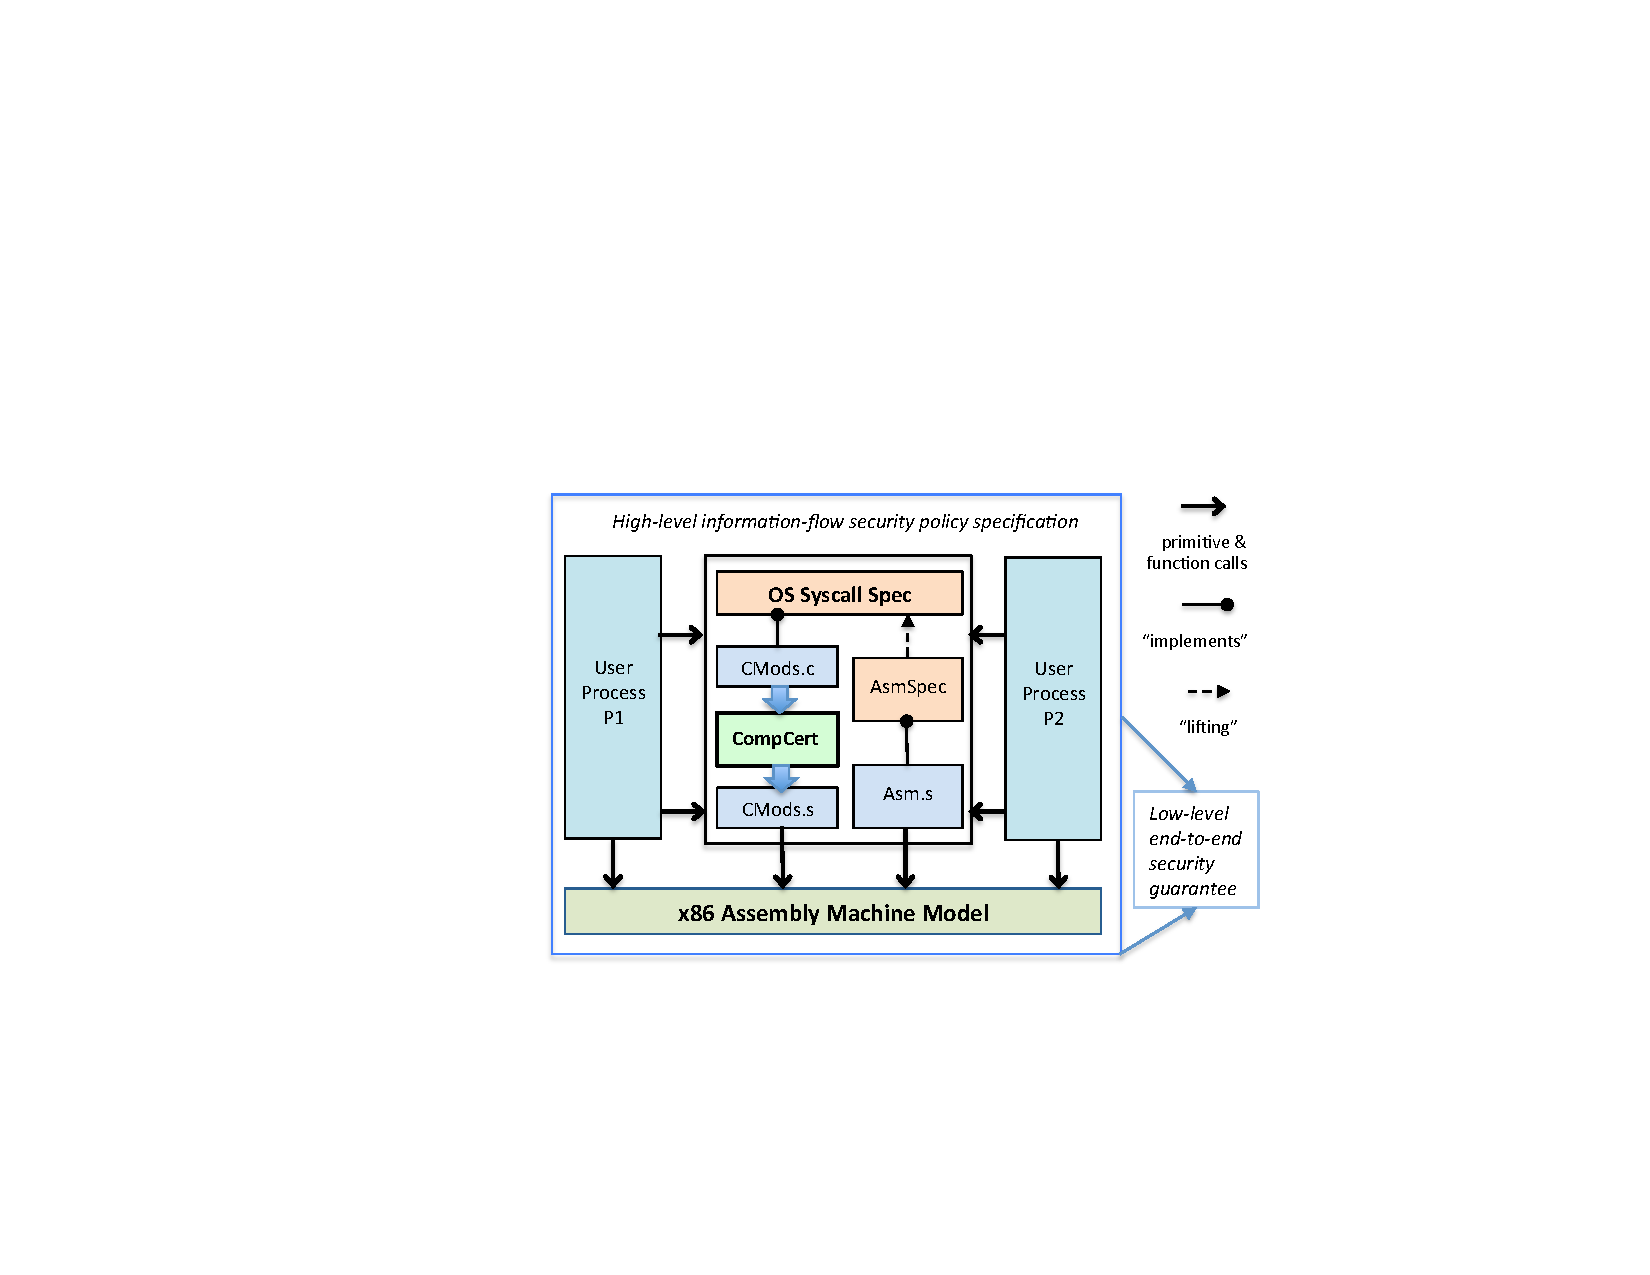
\includegraphics[scale=0.685]{pldi/figure/osmach}
\caption{\small An end-to-end software system that consists 
of both OS modules (in C and assembly) and user processes.}
\label{fig:osmach}
%\vspace*{-20pt}
\end{center}
\end{figure}
%%%%%%%%%%%%%%%%%%%%%%%%%%%%%%%%%%%%%%%%%%%%%%%%%%%%%%%%%%%%%%%%=

Security is desirable in today's real-world software.
Hackers often exploit software bugs to 
obtain information about protected secrets, such as user
passwords or private keys. A formally-verified end-to-end
security proof can guarantee such exploits will never be
successful. There are many significant roadblocks involved
in such a verification, however, and the state-of-the-art
is not entirely satisfactory.
 
Consider the setup of 
Figure~\ref{fig:osmach}, where a large system (e.g., an OS)
consists of many separate functions (e.g., system call primitives) 
written in either C or assembly. Each primitive has a verified
atomic specification, and there is a verified compiler, such as 
CompCert~\cite{compcert}, that can correctly compile C
programs into assembly. We wish to prove an \emph{end-to-end}
security statement about some context program (e.g., P1 or P2) that can call 
the primitives of the system, which ultimately guarantees that 
our model of the concrete execution (i.e., the whole-program assembly 
execution) behaves securely. This goal raises a number of 
challenges:
\begin{itemize}
\item \emph{Policy Specification}~--- How do we specify a clear
and precise security policy, describing how information is
allowed to flow between various domains? If we express the
policy in terms of the high-level syscall specifications, 
then what will this imply for the whole-program assembly execution? 
We need some way of specifying policies at different levels of 
abstraction, as well as translating between or linking separate 
policies.
\item \emph{Propagating Security}~--- It is well 
known~\cite{jurjens,morgan09} that
simulations and refinements may not propagate security guarantees.
How, then, can we soundly obtain a low-level guarantee from a 
high-level security verification?
\item \emph{Proving Security}~--- A standard way to prove
confidentiality is to formulate the property as noninterference,
and prove that some \emph{state indistinguishability} relation is
preserved by each step of execution (this is known as 
an \emph{unwinding condition}~\cite{goguen82,goguen84},
and will be discussed in Section~\ref{informal}). 
% this individual-step property
% is called an \emph{unwinding condition}~\cite{goguen82,goguen84}
% in the literature, and essentially serves as an induction
% hypothesis for proving whole-execution noninterference).
% In our setup, it is natural to express indistinguishability over
% abstract program states, and then prove security by verifying that 
% each primitive specification, taken as an atomic action, preserves
% the relation. 
However, this proof does not propagate down to the 
implementation: a syscall specification may atomically preserve
indistinguishability, but its non-atomic implementation may 
temporarily break the relation during intermediate states. Thus we
must be careful to formulate the security of a primitive's 
implementation as a global behavior-based property over the whole 
execution of the implementation, rather than a local state-based 
property over individual steps.
\item \emph{Cross-Language Linking}~--- Even if we verify security
for all atomic primitive specifications and propagate 
the proofs to implementations, there still may be incompatibilities
between the proofs for C primitives and those for assembly 
primitives. For example, a security proof for an assembly primitive 
might express that some data stored in a particular machine register 
is not leaked; this property cannot be directly chained with one for a 
C primitive since the C memory model does not contain 
machine registers. We therefore must support linking the
specifications of primitives implemented in different languages.
\end{itemize}
%%%%
In this paper, we present a novel methodology
for formally verifying end-to-end security of a system like the one
shown in Figure~\ref{fig:osmach}. First, security is proved for the
high-level specification of each syscall 
in a standard way, establishing noninterference
by showing that a state indistinguishability relation is preserved
across the specification. Then
we apply simulation techniques to automatically obtain a
sound security guarantee for the low-level assembly machine
execution, which is expressed in terms of whole-execution 
observations. Simulations are used both for relating specifications
with their C or assembly implementations, as well as for relating C 
implementations with their compiled assembly implementations.

The central idea of our methodology is to introduce a 
flexible definition of observation that unifies the concepts of 
policy specification, state indistinguishability, and 
whole-execution behaviors. For every level of abstraction, we 
define an \emph{observation function}
that % essentially 
describes which portions of a program state are 
observable to which principals. For
example, an observation function might say that ``$x$ is 
observable to Alice'' and ``$y$ is observable to Bob''.

Different abstraction levels can use different observation functions.
We might use one observation function mentioning machine registers to 
verify an assembly primitive, and a second observation function
mentioning program variables to verify a C primitive. These
observation functions are then linked across abstraction levels via
a special kind of simulation that preserves state
indistinguishability.


\ignore{
The following concepts can be formulated in terms of 
observation functions:
\begin{itemize}
\item \emph{Policy}~--- Given a principal $l$ and program state 
$\sigma$, an observation function induces a security policy
stating that there is no flow of information to $l$ from 
anything in $\sigma$ outside of 
$l$'s observation. In fact, we do not technically require 
observations to be a portion of program state; they can be any
arbitrary transformation on state. This allows us to express a
variety of security policies with % , including some kinds of 
declassification~\cite{sabelfeld-sands}. 
% We will present some examples of interesting 
% policies in Section~\ref{informal}.
\item \emph{Indistinguishability}~--- Two program states are
considered to be indistinguishable to $l$ just when $l$'s observations
on the states are identical.
\item \emph{Whole-Execution Observations}~--- Certain ``well-behaved''
types of observations, such as an append-only output buffer, can be 
used to describe global execution observations, or \emph{behaviors}. 
For example, an execution may have the behavior
``termination with final observation $o$''. We express security of 
the low-level system implementation in terms 
of whole-execution behavioral equality, since the high-level 
unwinding condition does not propagate across simulation.
\item \emph{Linking}~--- We use different observation
functions for different levels of abstraction. This means that we
can use an observation function mentioning machine registers to 
verify an assembly primitive, and a different observation function
mentioning program variables to verify a C primitive. These
observation functions are linked across abstraction levels via
a special kind of simulation that preserves state
indistinguishability.
\end{itemize}
}
%%%%
\begin{comment}
Note that none of these three aspects is individually novel. The
described security proof is a standard method for proving noninterference, 
known as \emph{unwinding}~\cite{goguen82,goguen84}.
The idea of preserving security across simulation or refinement has been 
explored in previous literature, such as~\cite{jurjens,morgan09,murray12}.
Expressing security policies in terms of an abstract notion of
observation or observable equivalence has also been 
explored~\cite{costanzo14,rhtt,sabelfeld99}. Our main contribution
in this work is to unify all three of these aspects with the \emph{single} 
concept of a general observation function. 
\end{comment}
%%%%
We demonstrate the efficacy of our approach by applying it to the mCertiKOS 
operating system~\cite{certikos-popl}. We modify mCertiKOS to disable all 
explicit inter-process communication, and then we prove noninterference between 
user processes with distinct IDs. mCertiKOS guarantees full functional correctness 
of system calls (with respect to an x86 machine model derived from
CompCert's model) by chaining simulations across many abstraction layers. We implement
our general notion of observation function over the existing simulation
framework, and then verify security of the high-level system call 
specifications. The result of this effort is a formally-verified security guarantee 
for the operating system~--- we specify exactly which portions of high-level state 
are observable to which processes, and we prove that the low-level 
model of assembly execution of the whole system is secure with respect to this 
policy. The security guarantee can be seen as \emph{end-to-end} in the following two ways:
(1) it applies across simulations, propagating from a top-level specification to a concrete 
implementation; and (2) it applies to whole-execution behaviors, guaranteeing that an 
entire execution is secure from start to finish. 

\cut{
Note that, while most of the mCertiKOS code is written in C and compiled into
assembly by CompCert, there are some primitives that must be written directly
in assembly. Context switch is a classic example of such a primitive.
The primary functionality of a context switch 
involves copying values between machine registers and kernel objects;
hence both the implementation and specification of the primitive 
must refer to low-level machine state. A key goal and contribution of
our security verification is that assembly primitives like context
switching are fully handled within the framework, and thus do not need to
be trusted.}

\vspace{2mm}
\noindent
To summarize, the primary contributions of this work are:
\begin{itemize}
\item A novel methodology for end-to-end security verification of 
software systems written in both C and assembly, and extending across various
levels of abstraction.
\item An end-to-end security proof, completely formalized in the
Coq proof assistant~\cite{coq}, of a simple but nontrivial operating system
kernel that executes over an extension of the CompCert x86 machine model.
The kernel is non-preemptive, and explicit communication between processes 
is disabled.
\end{itemize}

%\paragraph{Paper Organization}
The rest of this paper is organized as
follows. Sec.~\ref{informal} introduces the
observation function and shows how to use it for policy
specification, security proof, and linking.
Sec.~\ref{methodology} formalizes our simulation framework and
shows how we prove the end-to-end security theorem. 
Sec.~\ref{casestudy-def} and~\ref{casestudy-proof} describe the
security property that we prove over mCertiKOS, 
highlighting the most interesting aspects of our proofs. 
Sec.~\ref{limitations} discusses limitations, assumptions,
and applicability of our methodology. Finally, Sec.~\ref{related}
discusses related work and concludes.

\ignore{


\begin{comment}
The first task took approximately three person-months,
and the second took two person-months.
\end{comment}

\begin{comment}
Consider the setup of Figure~\ref{compile}, where we have an abstract 
specification of a C program, and a compilation of the C program down 
to assembly code. Assume that we have verified two simulations connecting
the specification to the C program, and the C program to the assembly
program.




design a methodology for proving security that
can cleanly support all of the following aspects:
\begin{itemize}
\item \emph{General Policies}~--- It must be easy to define how
state is divided into security domains, how information is allowed
to flow between these domains, and how declassifications can occur.
\item \emph{Application to Low-Level Code}~--- We must have an
end-to-end property that applies to the actual code of the software,
which may be written in C or even assembly.
\item \emph{Tractable Proof Effort}~--- The amount of human effort
required to actually construct the proof must be reasonable.
\end{itemize}
There are many existing frameworks and methodologies for
formally proving security, but none of them satisfactorily
support all of our desired properties. These properties
are often at odds with one another; for example, cleanly
defining security policies requires a high level of abstraction,
and is thus difficult to reconcile with low-level code.

In this work, we will focus on the formal verification
of security for low-level code, such as the C and assembly code that
implements an OS kernel, by leveraging the power of simulation.

We achieve our goal in the following way:
\begin{enumerate}
\item We define security in terms of a highly abstract notion of 
a state observation function. General security policies can be presented 
using this observation function.
\item We define a specialized form of simulation that preserves 
state indistinguishability between machines, as defined by the observation
function. These simulations allow different machines to have different
definitions of observation.
\item We prove that our specialized simulations preserve security: if an
execution of the top-level machine is proved to be secure, then the 
corresponding execution of the bottom-level machine is guaranteed to be secure.
\end{enumerate}
\end{comment}


\begin{comment}
To get a better sense of our approach and its contributions, we will now
discuss how our approach handles two tricky aspects of security verification.

\subsection{Hiding Confidential Data via Atomicity}
\label{hiding}

The following discussion is not novel to our methodology, but rather 
provides some context justifying our choice to prove security at
a high level of abstraction. Let us start with an informal description
of security (confidentiality). Assume we have a type for 
program state and some particular principal (or security domain)
called the \emph{observer}. Our security property will then be 
parameterized by an \emph{observation function} which takes a state 
and returns some part of the state that is known to the observer.
We say that two states are \emph{indistinguishable}, or observably 
equivalent, just when the observations on those states are equal. A 
\emph{secure action} is then a state transition that always takes 
two indistinguishable states to two other indistinguishable states.
Intuitively, secure actions do not leak any information about the
unobservable part of the state. We say that a program is secure
when its semantics, taken as a single big step, constitutes a
secure action.

Note that this definition of security can support some
kinds of declassification policies simply by extending the
observation function. As a very basic example, we can
allow the parity of some high-security data to be declassified
by proving that an action is secure with respect to an observation
function that transforms the high-security data into its
parity. In other words, the action will have the same observable
behavior on any two states in which the high-security data has
the same parity. This semantic and relational view of declassification
is used in some other security-reasoning frameworks such 
as~\cite{sabelfeld99,rhtt,costanzo14}. 

It is trivial to show that secure actions compose sequentially.
This means that we can always prove a program secure by proving
that each individual step of the program is secure. Many existing
security-reasoning frameworks use this strategy. For example,
many typed-based approaches~\cite{jif,hritcu13,slam,austin09} assign security
classifications to program variables (either statically or dynamically),
and then show that each step of the program obeys a policy preventing
information flow from higher classification levels to lower ones.
Some language constructs such as conditional branching must be treated
with care to avoid implicit flows.

This strategy for security verification is unfortunately incomplete,
however, as it necessarily rules out programs that
perform some insecure actions but hide these insecurities
from the observer. As a rather trivial example, the strategy cannot support 
the following simple C program, consisting of an unobservable
global variable~\ttt{password} and an observable global 
variable~\ttt{public}:
\begin{alltt}
  public = password;
  public = 0;
\end{alltt}
This program is atomically secure since it immediately forgets the secret 
data that it read. A line-by-line analysis, however, will not be able
to prove the security of this program since the first line directly
violates security. If an observer reads~\ttt{public} at the point of execution
that occurs in between the two lines of code, then the secret is leaked. 
There are a number of ways to support this type of example, including 
attaching security labels to data instead of locations, and enforcing 
information erasure policies~\cite{chong05}. In this work, we
advocate proving the security of this type of program by abstracting
the program into an atomic specification, and then proving that
the specification is secure.

Note that while this particular example is not something that one would
ever want to write in a real system, we will describe a realistic example
of hiding a potential security leak in
Section~\ref{casestudy-proof}. The example is the implementation of
the page-fault handler in the mCertiKOS kernel. The handler must
allocate a new page and obtain this page's physical address, a value
which could potentially be abused to violate security.  However, the
handler is careful not to make this physical address observable; it is
used only to map the page into the current process's virtual address
space, and then the physical address is forgotten (from the observer's
point-of-view).

While abstracting a program into an atomic action simplifies the security 
proof, it does not solve the whole problem. After all, one of our goals
is that the security proof applies to low-level code~--- the actual
implementation, not the abstract specification. As discussed with the above
example, there is no hope for our security property to hold on each
individual step of the implementation; the steps may be locally insecure. 
Instead, we will prove a global notion of security for the actual 
implementation. While the observation function can refer to any portion
of program state in the abstract specification, we will require that 
implementation uses a different observation function that resembles an
output buffer, or the observer's monitor. More precisely, we will require
a monotonicity property on the observation function of the implementation,
saying that once data is made observable, it can never be made unobservable
later. In the context of the above example, we are essentially saying that
the value of variable \ttt{public} is not what the observer actually sees;
instead, the language should include an explicit print command to 
convert ``observable'' data into ``observed'' data. We will explain and 
formalize this point more clearly in Section~\ref{methodology}. The 
most important thing to see here is that the observation function of the 
specification is \emph{not} required to be monotonic, and can therefore
still express a wide variety of interesting security policies.

\subsection{Security-Preserving Simulation}

Our work represents, to the best of our knowledge, the first disciplined 
approach to preserving security across many layers of simulation. There 
have been other works that addressed the problem of preserving security 
across refinement~\cite{morgan09,jurjens}, including the closely-related
security verification of the seL4 kernel~\cite{murray12}. According
to Lynch's definition~\cite{Lynch95}, a refinement is a special case
of simulation where the simulation relation is a function (i.e., each
state in the higher-level machine is related to exactly one state in
the lower-level machine). Our work aims to preserve security across
arbitrary forward simulations, not just refinements. Indeed, the mCertiKOS
simulations sometimes make use of one-to-many simulation relations
(e.g., abstracting a list into an unordered set).

\begin{figure}
\centering{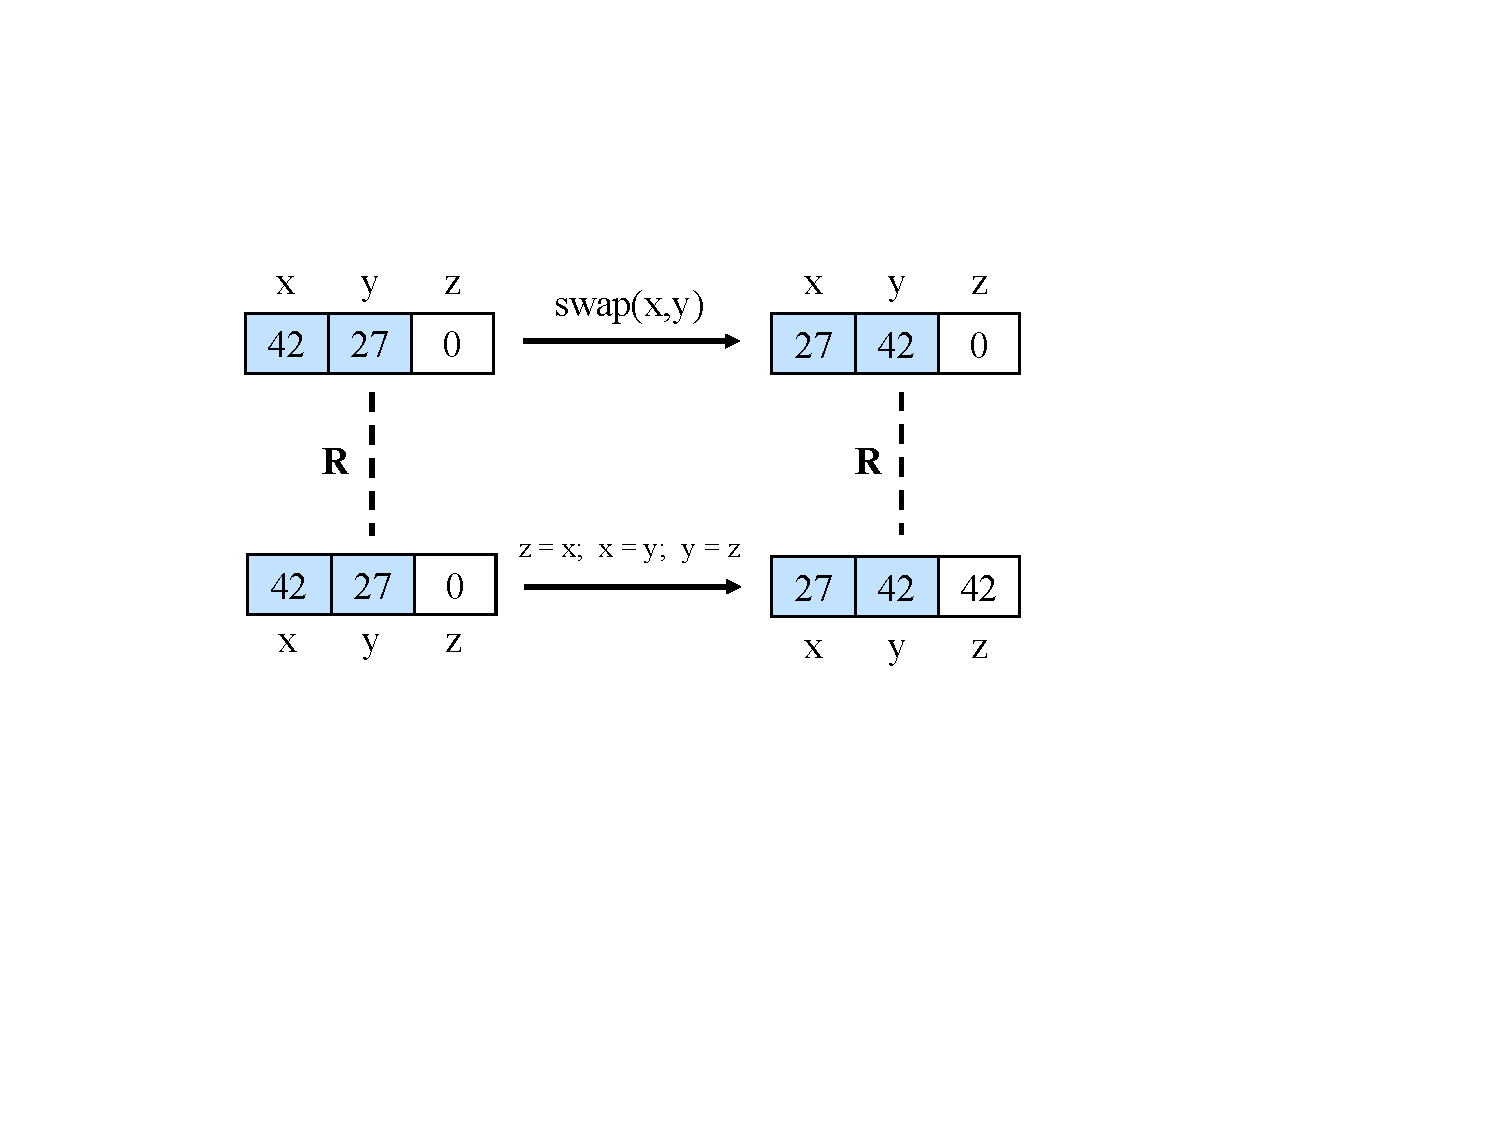
\includegraphics[scale=0.6,origin=c]{figure/paradox.pdf}}
\caption{\small{Security-Breaking Simulation: both the specification 
and implementation executions are deterministic, yet $R$ causes the 
implementation to be insecure as it relates $y$ to any value.}}
\label{paradox}
\end{figure}

When using refinement, security may not be preserved only when a 
nondeterministic program is refined into a more deterministic one. When 
using general simulations, however, even secure deterministic programs can
be simulated in an insecure way. Figure~\ref{paradox} illustrates this
point. The example assumes a program state consisting of a high-security 
(unobservable) variable $x$ and low-security (observable) variable $y$. 
The abstract action (specification) writes $0$ into $y$, while the concrete 
implementation writes $x$ into $y$. The relation $R$ relating abstract to 
concrete states simply requires that $x$ has the same value in the two 
states, and $y$ always has value $0$ in the abstract state (hence the
relation is one-to-many). It is easy to show that $R$ is a valid simulation
relation for this example (in fact, it is a valid bisimulation
relation). The abstract action is clearly secure,
as the final value of $y$ is guaranteed to be $0$ and thus has no 
dependency on the secret value of $x$. However, the implementation
is not secure: the final value of $y$ clearly depends directly
on $x$. Using the terminology above, the state observation is the value
of $y$; the abstract program always takes two indistinguishable initial 
states to indistinguishable final states, while the concrete one may not.

Our solution to this issue is obvious but fundamental. The simulation in
Figure~\ref{paradox} breaks security because security talks about 
indistinguishability of states, yet the relation $R$ fails to 
preserve indistinguishability. We therefore define a notion of
``indistinguishability-preserving simulation'', which is a normal
simulation with the additional property that two indistinguishable
states are always related to indistinguishable states. We will formalize
this in Section~\ref{methodology}, and prove that such a simulation
preserves security.

%\vspace{2mm}
\noindent
To summarize, the contributions of our work are as follows:
\begin{itemize}
\item We present a novel methodology for proving security based on
layered simulations. The security proof is done at the most
abstract layer, and can therefore express interesting policies,
including some kinds of declassification. The simulations are
specialized to preserve security, so that an
end-to-end property still holds over the most concrete layer.
No security reasoning is required over any layer besides the
abstract one.
\item We demonstrate the effectiveness of this methodology with
a major proof effort: the confidentiality between user-processes
executing over the mCertiKOS~\cite{certikos-popl} kernel.
Like mCertiKOS, our proof is fully formalized in the Coq proof 
assistant~\cite{coq}, and the code can be found in the supplementary
material~\cite{costanzo-popl16-tr}.
\end{itemize}
\end{comment}

\begin{comment}
Now that we have described our methodology for proving security,
let us revisit the initial goals:
\begin{itemize}
\item \emph{General Policies}~--- 
The observation function allows us to specify interesting security 
policies at an arbitrarily high level of abstraction. We will 
present many example policies in Section~\ref{policies}. 
\item \emph{Application to Low-Level Code}~--- 
Our solution to the refinement paradox (restricting the simulation
relation according to observations)
allows us to propagate a high-level security policy to the actual 
low-level execution.
\item \emph{Tractable Proof Effort}~--- The required proof effort is 
reasonable, as it is divided into the two
orthogonal tasks of abstracting code into a functional specification, and
then proving security over the specification. The security proof only
requires showing that single steps preserve observable equivalence;
multi-step reasoning follows automatically from induction.  
Functional specifications can be reused for proving other properties 
besides security. In Sections~\ref{casestudy-def} and~\ref{casestudy-proof}, 
we support our claim 
that the proof effort is reasonable by presenting a full security proof 
over a variant of the mCertiKOS kernel.
\item \emph{Completeness}~--- Our proof strategy achieves a satisfactory 
level of completeness, since it allows for proving an entire program secure 
even when the program manipulates data in a locally insecure way.
\end{itemize}
\end{comment}

\begin{comment}
\subsection{Security Verification of mCertiKOS}

In Sections~\ref{casestudy-def} and~\ref{casestudy-proof}, we
demonstrate our security proof methodology with a large-scale,
practical example. We prove a security property over a version of the
mCertiKOS kernel, stating that user processes are isolated from each
other. The proof is developed entirely within the Coq proof assistant,
and thus is machine-checkable.

The first step of the proof~--- abstraction of system call
implementations into functional specifications~--- was already
completed by Gu~{\em et al}~\cite{certikos-popl}. The proof presented
here deals with the second step: specifying a security policy
(observation function) and proving the security property instantiated
with this policy. While the abstraction step took about $1.5$
person-years (including the time for developing much of the refinement
framework), the security step took only $3$ person-months to complete.

To the best of our knowledge, our work is only the second
fully-formalized OS security proof to be completed; the first is the
verification effort over the seL4 
kernel~\cite{klein14,sewell11,murray12,murray13}.
There are some major shortcomings in the seL4 effort, however, that
our methodology allows us to address. One shortcoming comes from the
fact that the seL4 proof uses standard refinement rather than
contextual refinement.  This means that malicious user code (context
code) could potentially interfere with kernel state in such a way that
the refinement becomes unsound. Indeed, the seL4 security proof needs
to assume that user-level actions only touch a portion of memory state
isolated from the kernel (the user's virtual address space). In our
security verification over mCertiKOS, we \emph{prove} that users'
actions are correctly isolated to their virtual address spaces.

A second shortcoming of the seL4 proof is that it does not deal with
page faults in their model of user-level
transitions~\cite{klein14,daum14}; this is a severe limitation since
virtual memory without page fault handling would be almost unusable.
As we will show later in Section~\ref{ssec:oprim}, the security of the
page-fault handling primitive is one of the hardest and the most
tricky components in our security verification over mCertiKOS.

A third shortcoming of the seL4 proof is that their state simulation
relation is the identity relation. This means that, while they can abstract
code into atomic specifications, they cannot abstract machine state 
into more convenient forms or into purely logical state. Not only
does this make the functional specifications difficult to present
in a readable way, but it also limits the expressiveness of security 
policies. Note that they completely elide the refinement
paradox issue by never abstracting program state.

A fourth issue with the seL4 proof is that refinement is only verified
for implementations written in C. Anything written directly in
assembly is assumed to have been implemented and abstracted correctly.
This is particularly relevant for an operating system, since there is
some functionality such as context switching that \emph{must} be
implemented in assembly. Our contextual refinement framework, on the
other hand, guarantees that the functional specification is a correct
abstraction of the actual implementation, regardless of whether the
implementation is written in C or assembly. Thus we can be certain
that our security theorem propagates down to the actual
implementation, even across assembly primitives like context switch.
\end{comment}

}
